\subsection{Ejercicio 13}
\graphicspath{ {img/13} }

\subsubsection{Proceso aceptar cookies necesarias}

Según la Agencia Española de Protección de Datos, los sitios web deben ofrecer al usuario la posibilidad de aceptar o rechazar las cookies no necesarias de forma clara y sencilla, sin que aceptar las cookies sea más fácil que rechazarlas \cite{AEPD}. Teniendo esto en cuenta, consideramos que los tres sitios web mencionados deberían permitir aceptar solamente las cookies necesarias.

Las políticas de cookies de los sitios web son:
\begin{itemize}
    \item \url{https://www.udc.es/es/pe/cookies/}
    \item \url{https://www.lavozdegalicia.es/docs/politica_de_cookies.htm}
    \item \url{https://www.marca.com/cookies.html}
\end{itemize}

La política de cookies de la Universidad da Coruña (UDC), que también se aplica al catálogo CRUNIA, menciona que se pueden "restringir, bloquear o eliminar" manualmente las cookies no necesarias desde la configuración de tu propio navegador, teniendo en cuenta que no se podrá hacer uso de algunas funcionalidades indicadas en las propias cookies.  

\begin{figure}[H]   
    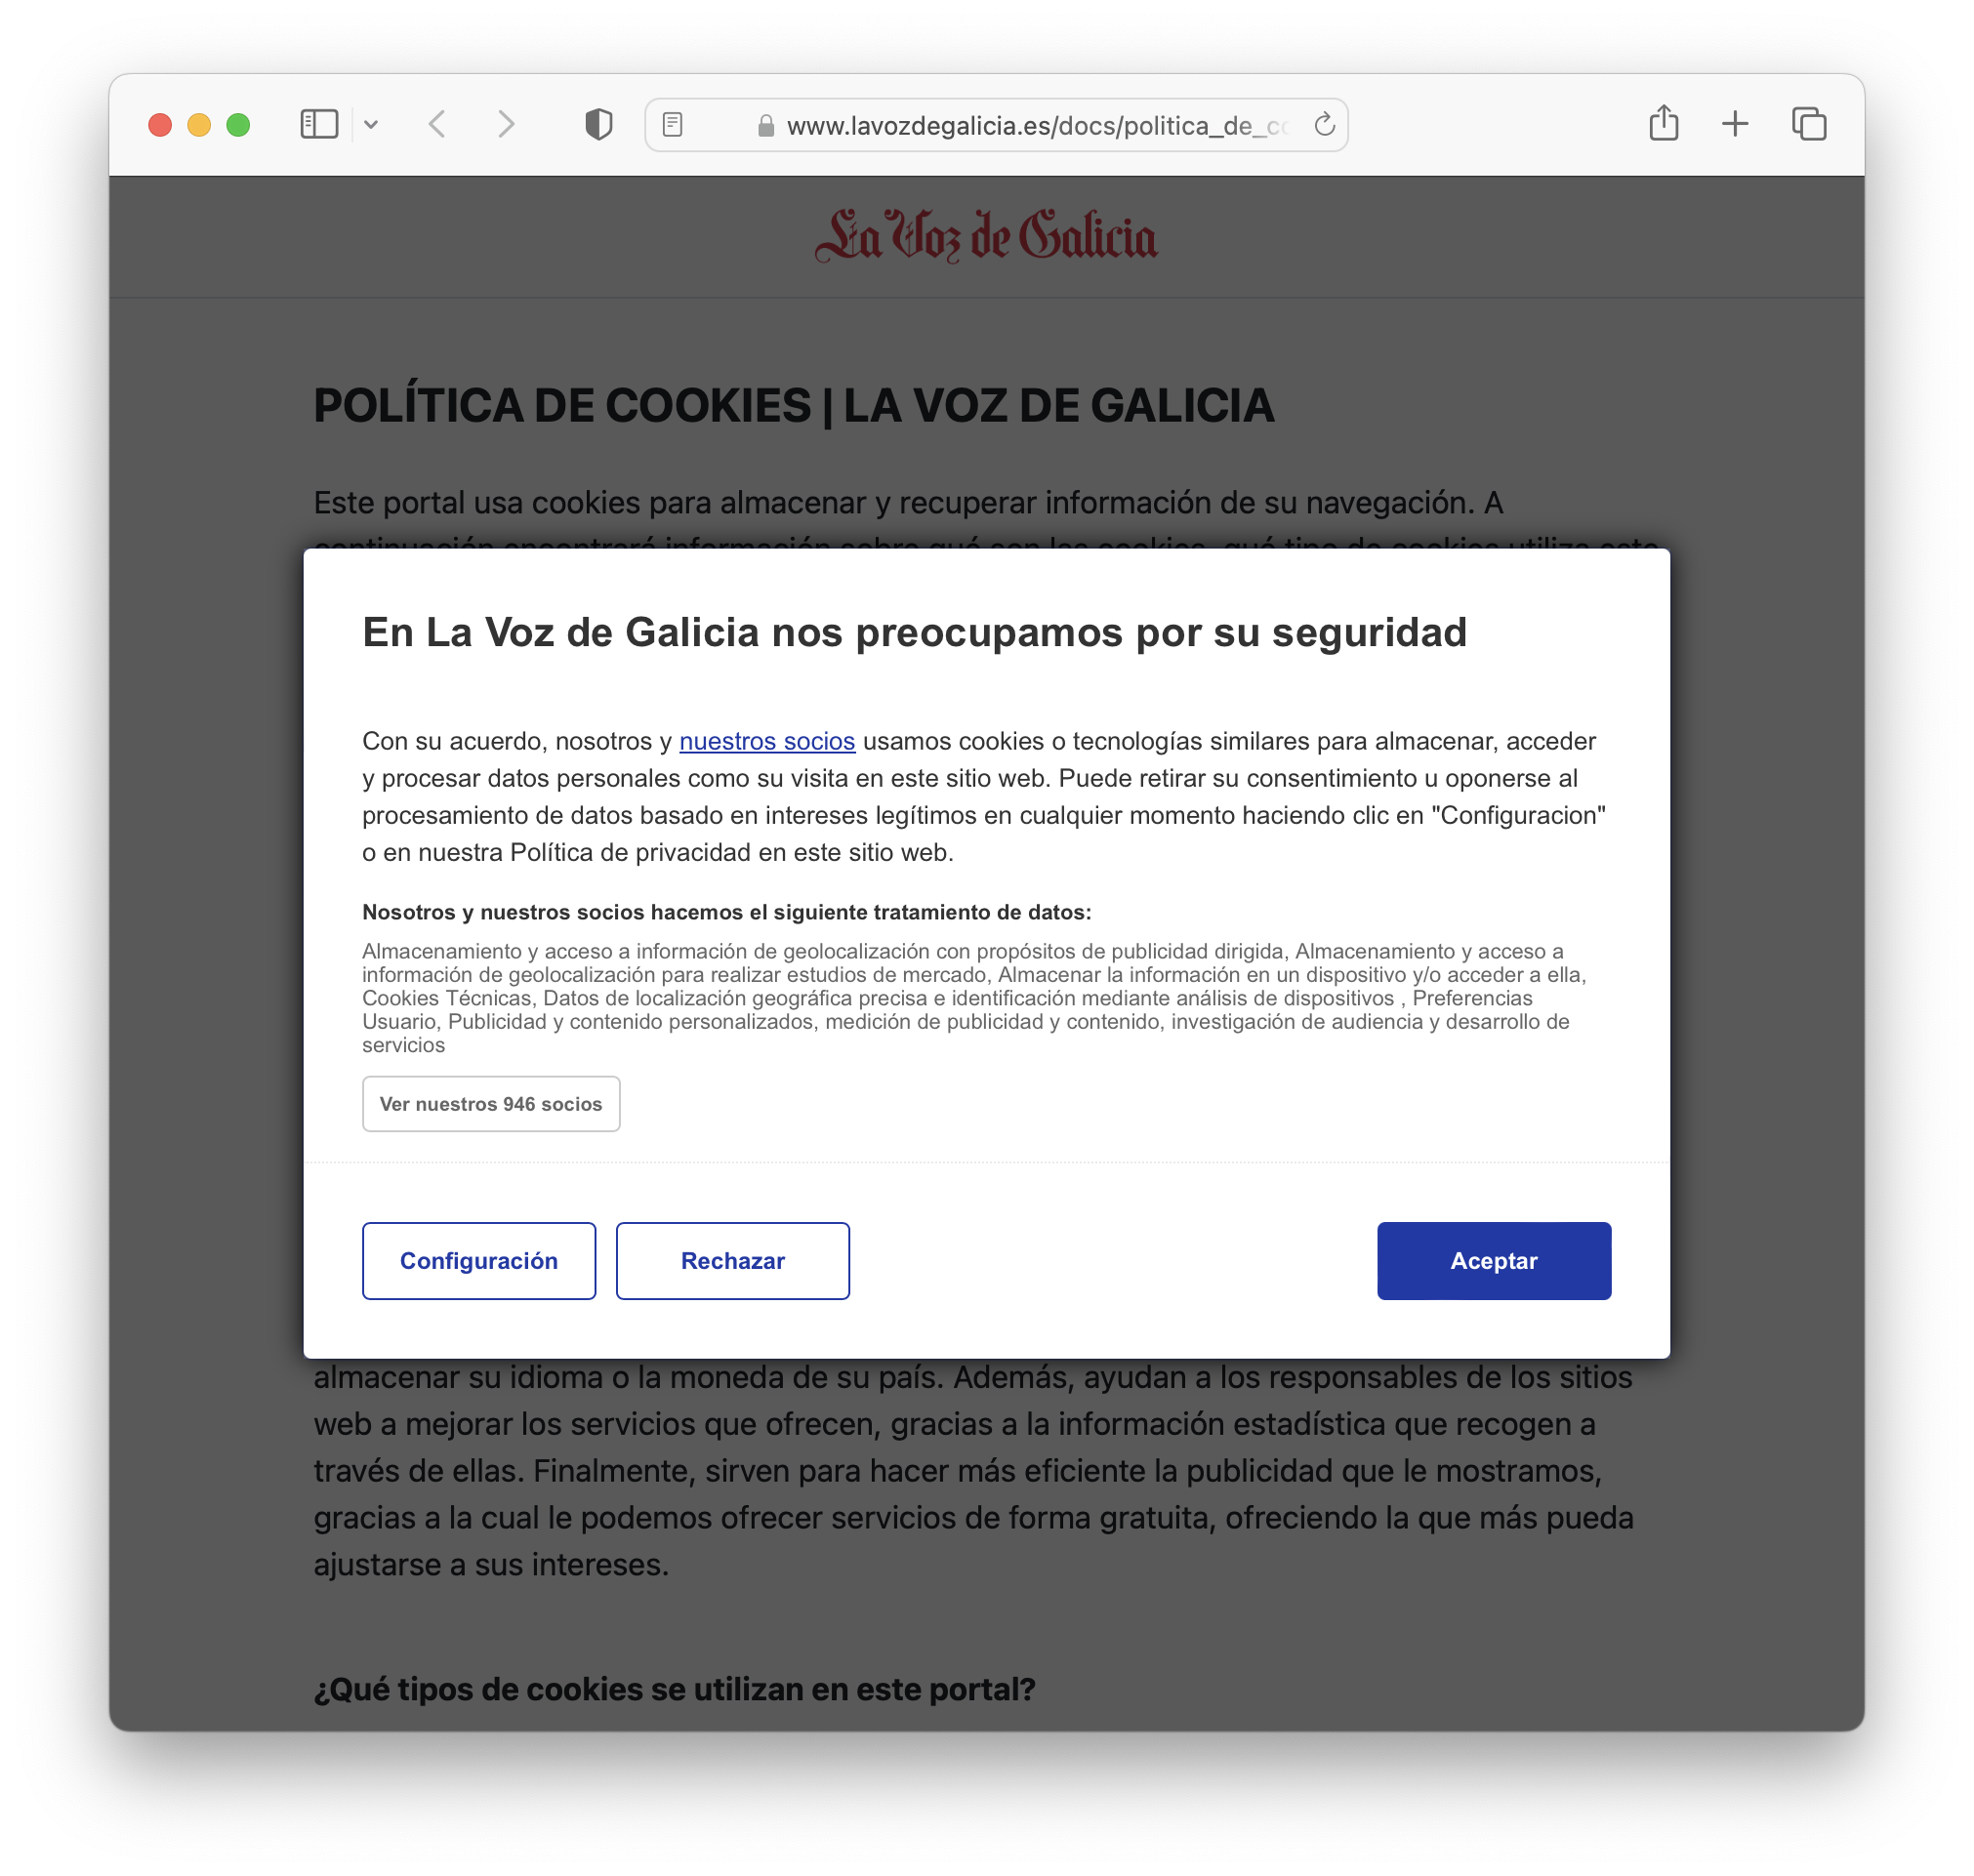
\includegraphics[width=15cm]{cookies_voz.png}
    \caption{Aviso cookies inicio La Voz de Galicia}
    \label{fig:cookies_voz}
\end{figure}

En el sitio web de La Voz de Galicia, al acceder por primera vez, como se ve en la \ref{fig:cookies_voz}, se presenta un aviso de cookies que permite al usuario gestionar sus preferencias de manera personalizada. Este aviso ofrece la opción de aceptar todas las cookies o configurar cuáles se desean aceptar, incluyendo la posibilidad de rechazar las cookies no esenciales. 

Para aceptar únicamente las cookies necesarias, el usuario debe seleccionar la opción de configuración y desactivar las categorías de cookies no esenciales, como las de análisis estadístico, geolocalización o publicidad comportamental. Este proceso, aunque requiere varios pasos, está diseñado para ser claro y accesible, cumpliendo con las directrices de la Agencia Española de Protección de Datos. 

Además, la política de cookies de La Voz de Galicia detalla los tipos de cookies utilizadas y proporciona enlaces a las políticas de privacidad de terceros involucrados, como Google Analytics, Chartbeat o Facebook. Esto permite al usuario tomar decisiones informadas sobre su privacidad y el uso de sus datos personales. 

\begin{figure}[H]   
    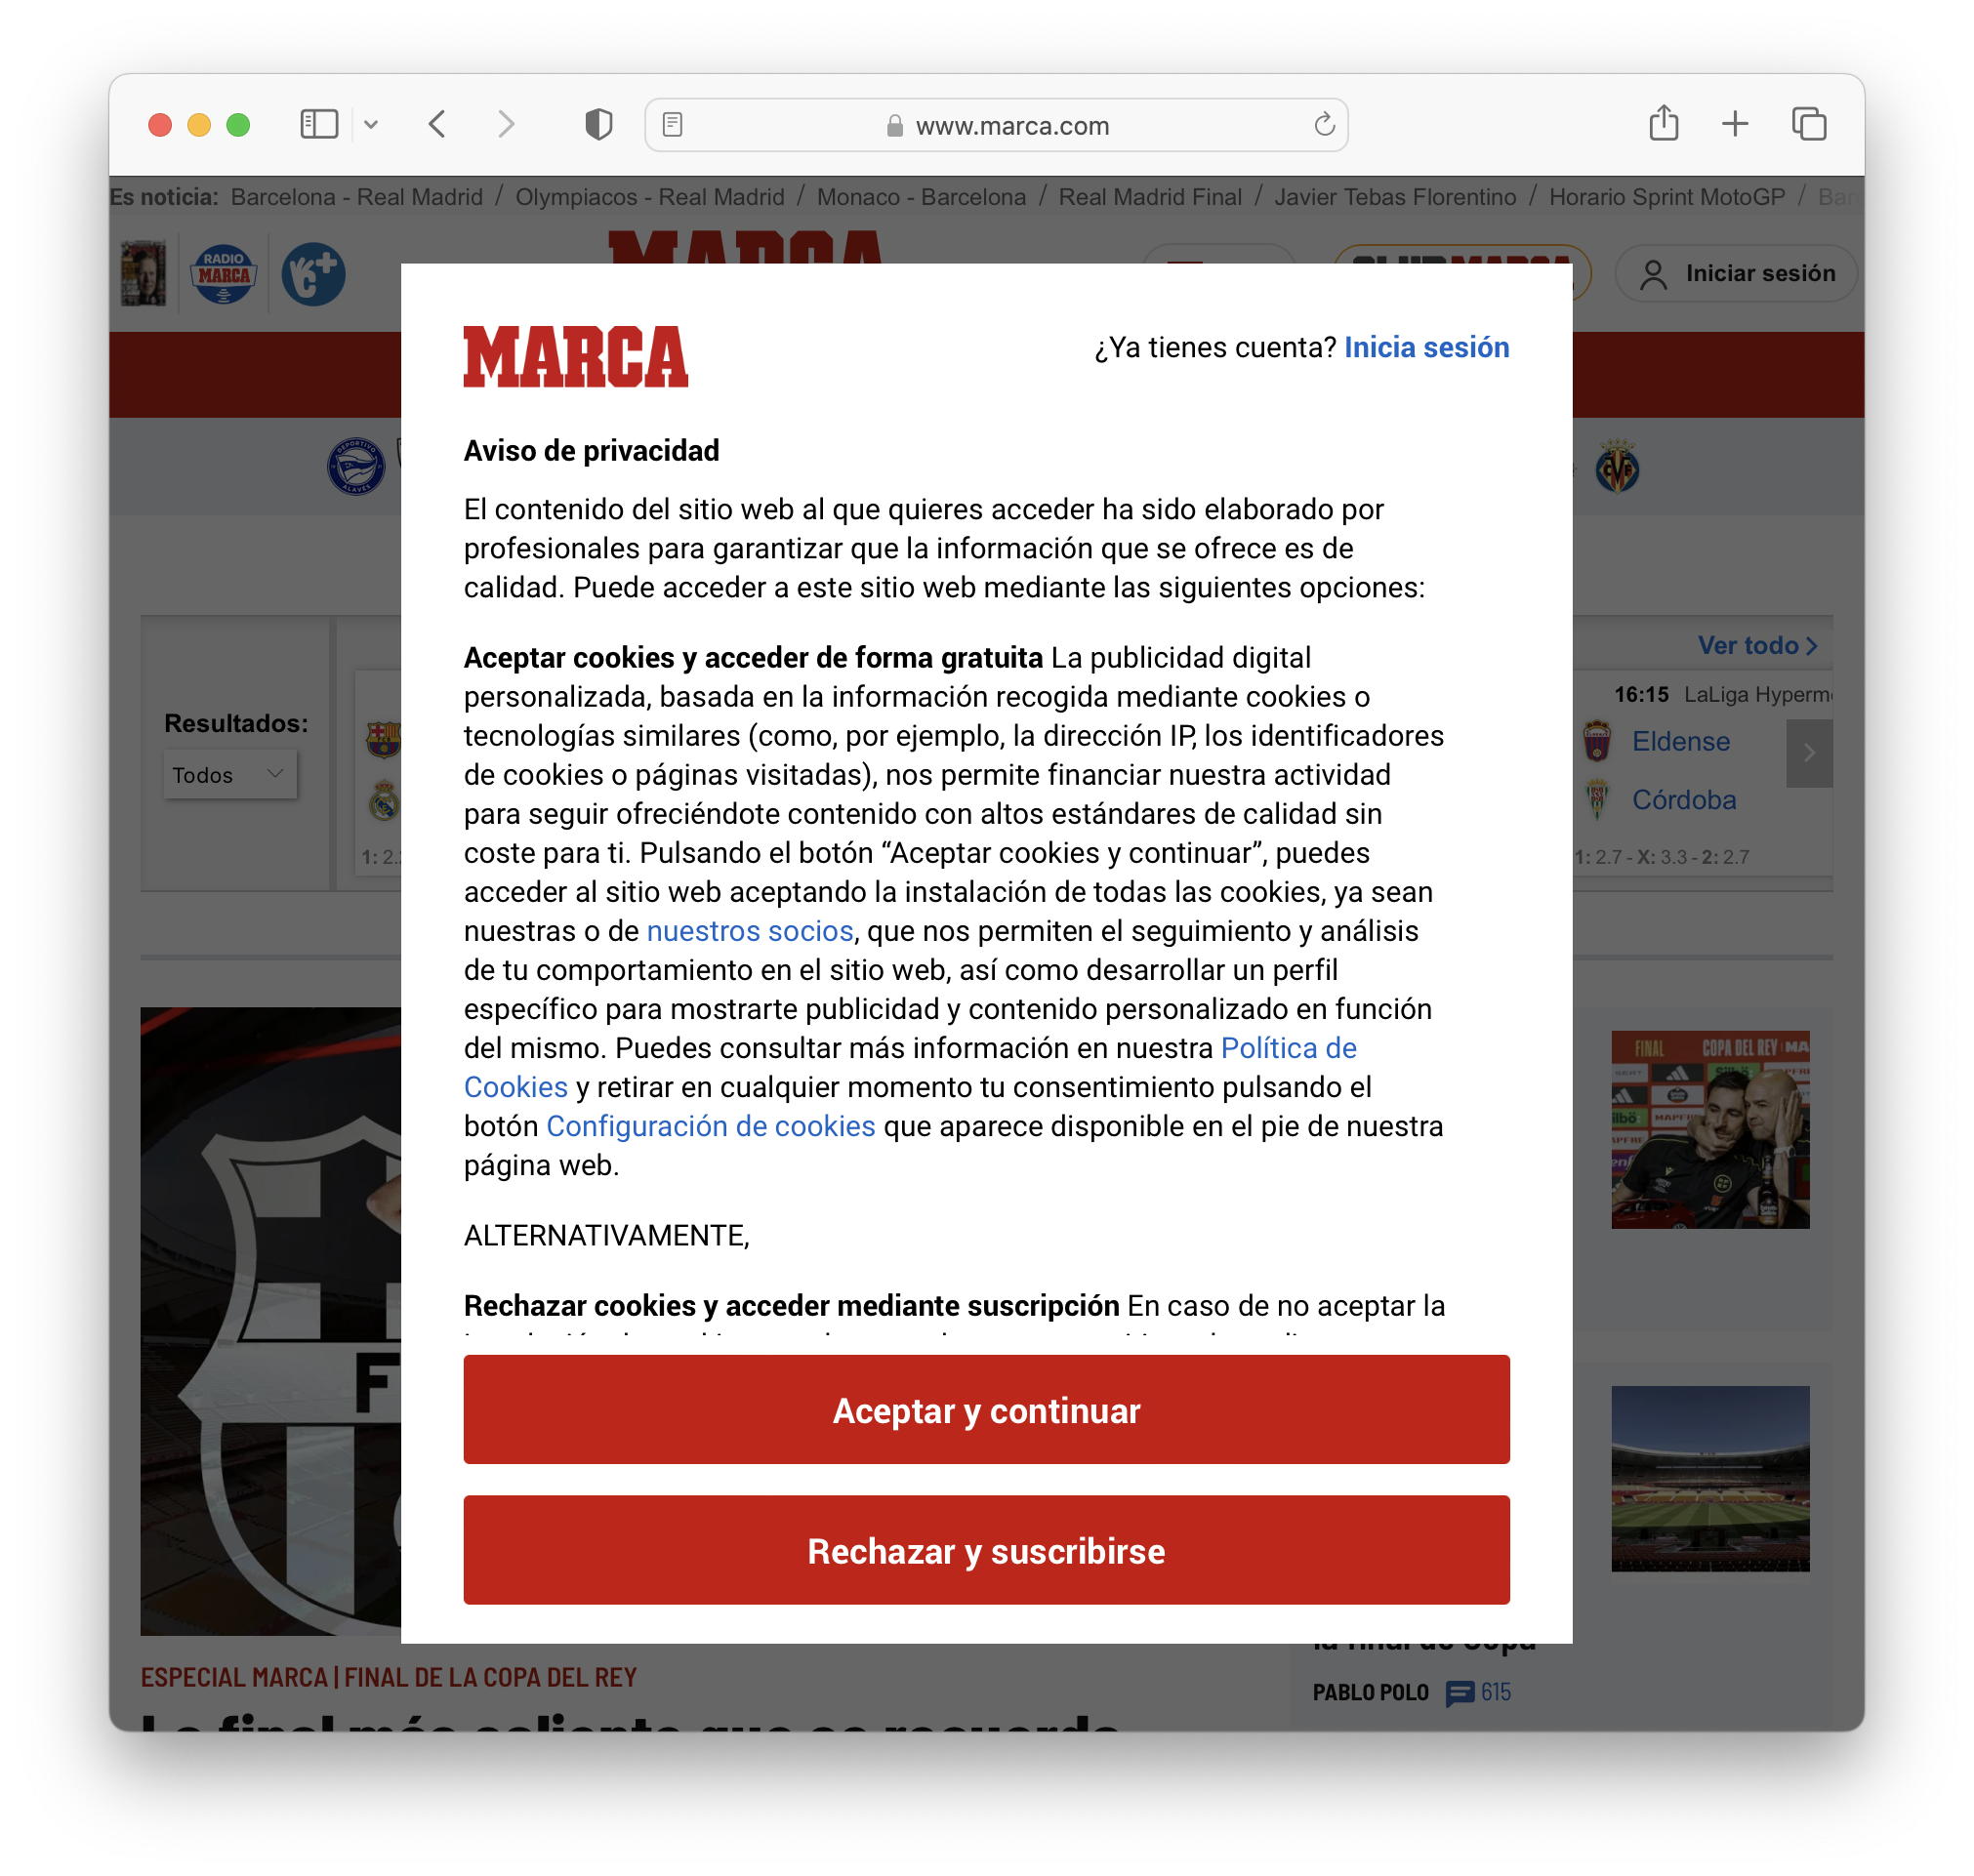
\includegraphics[width=15cm]{cookies_marca.png}
    \caption{Aviso cookies inicio MARCA}
    \label{fig:cookies_marca}
\end{figure}

\begin{figure}[H]   
    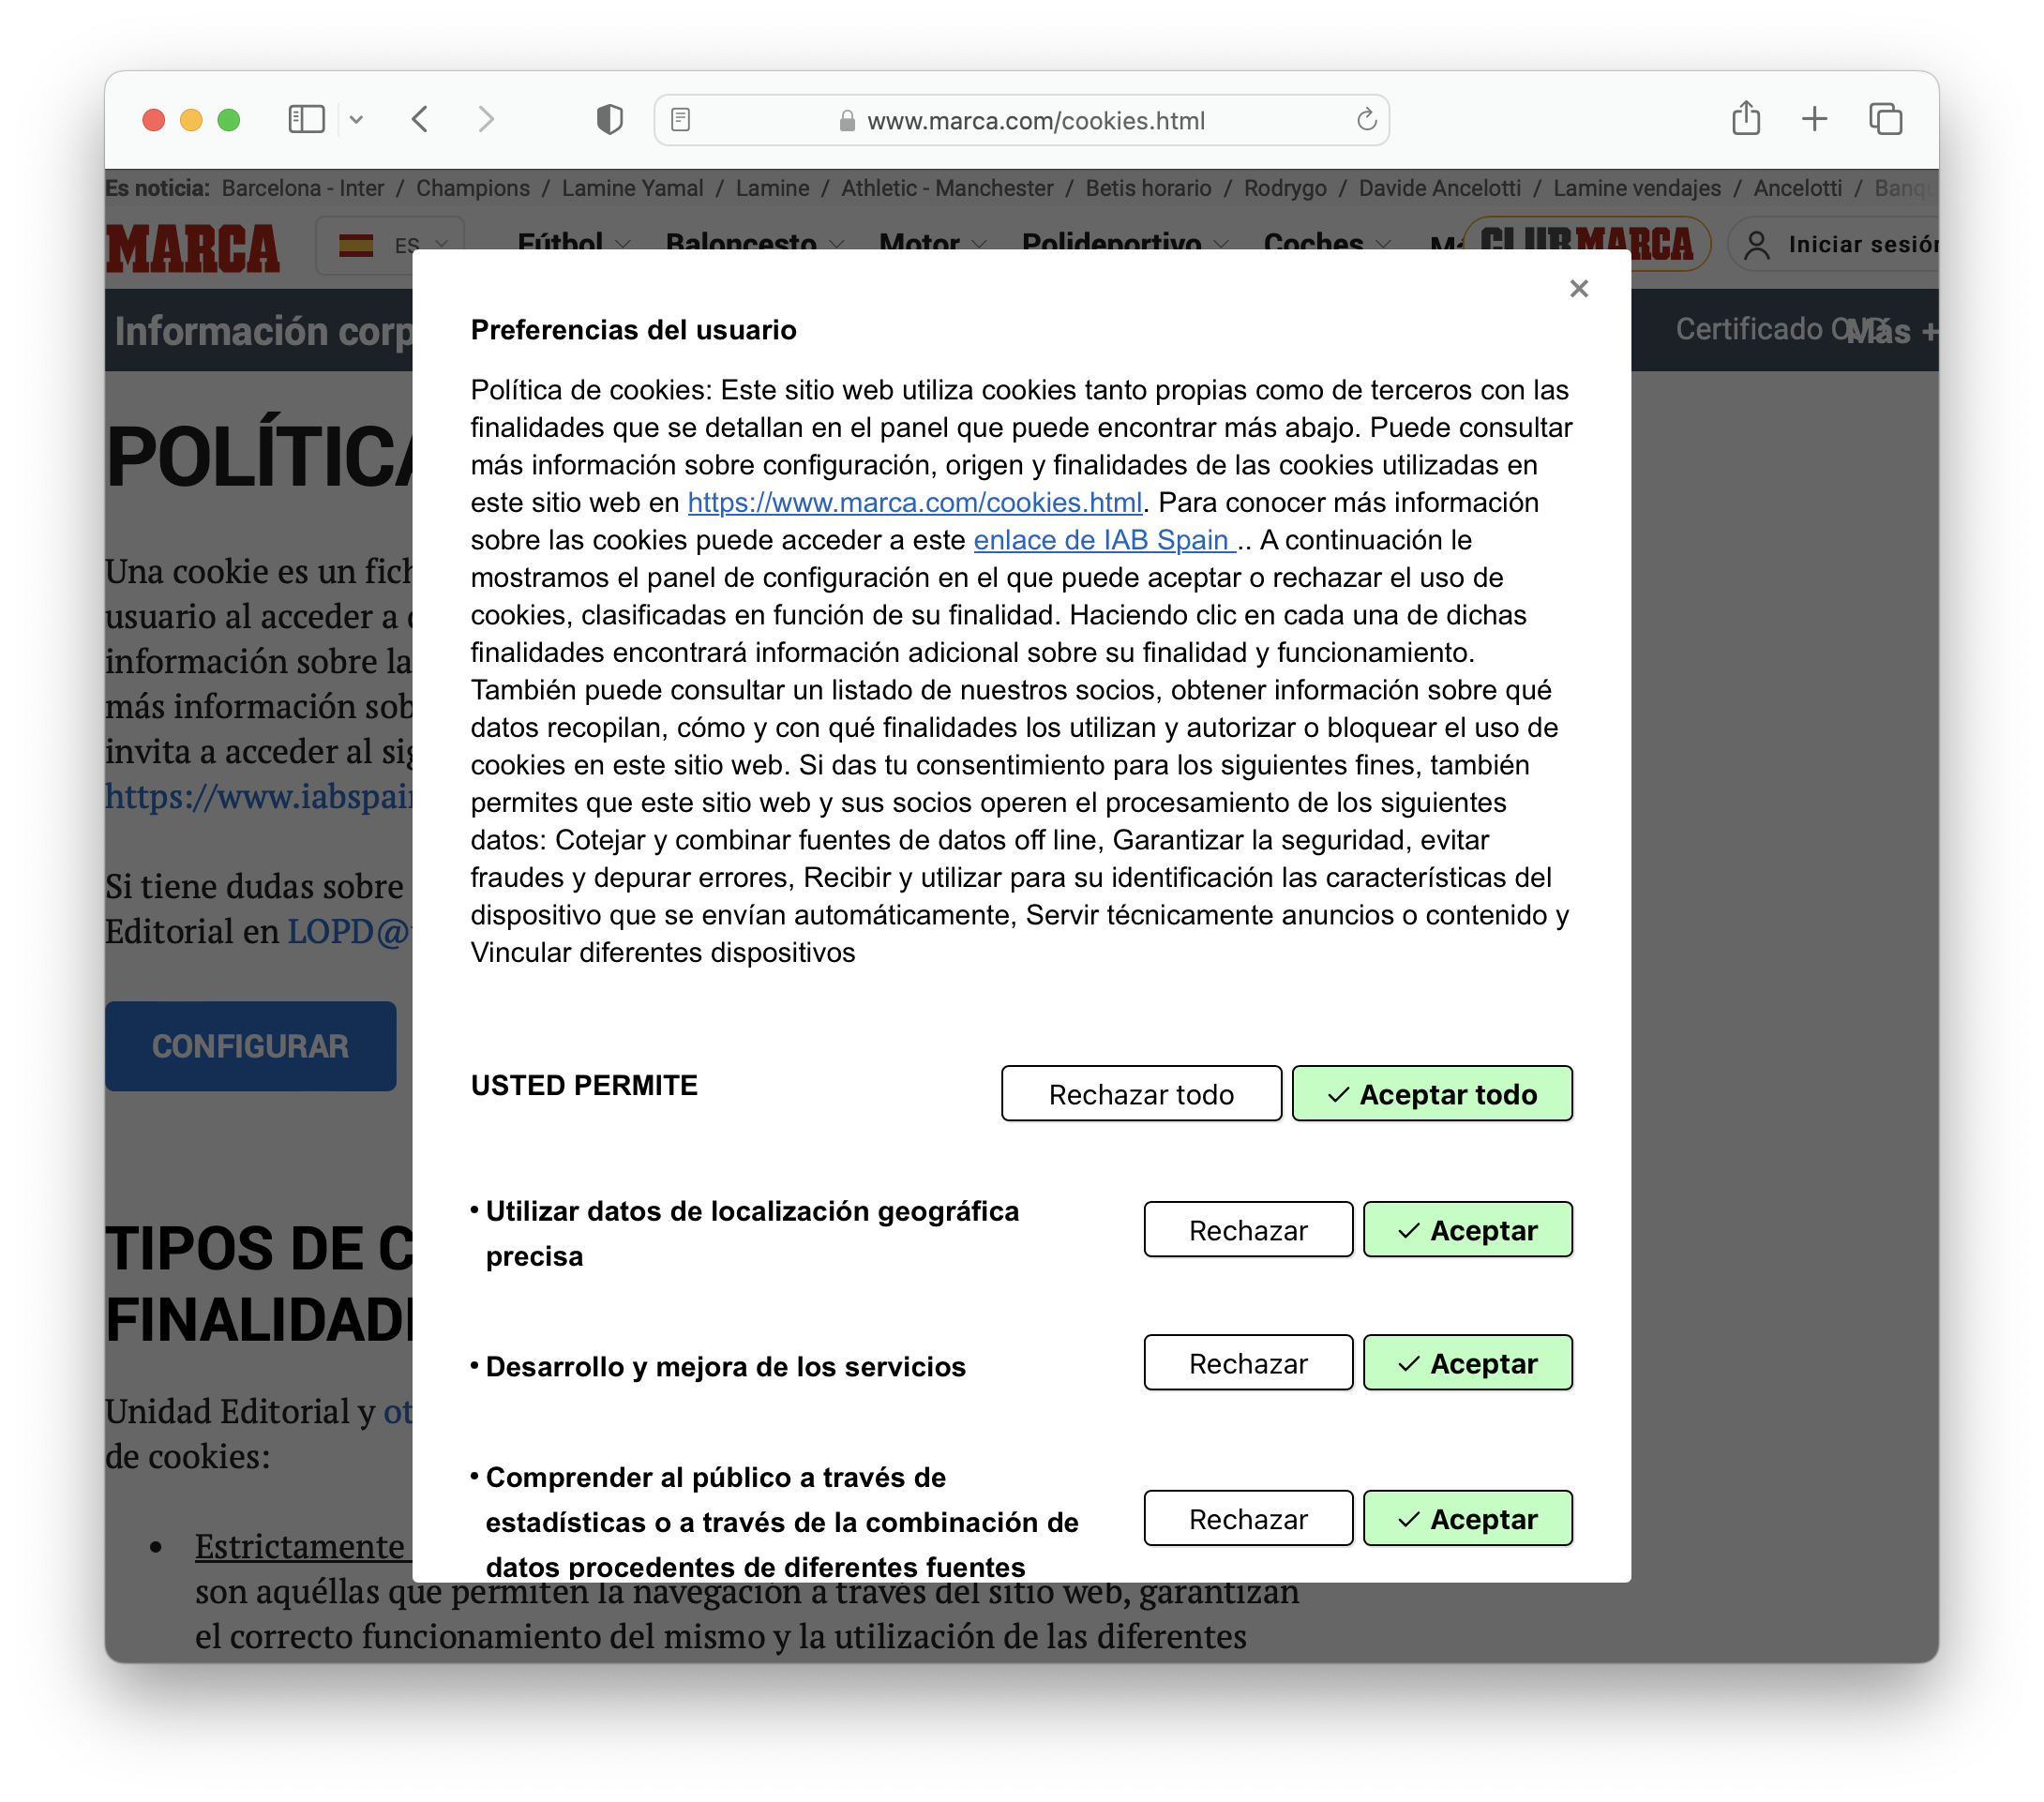
\includegraphics[width=15cm]{panel_cookies_marca.png}
    \caption{Panel configuración cookies MARCA}
    \label{fig:panel_cookies_marca}
\end{figure}

Tal y como sucedía en La Voz de Galicia, en el sitio web de MARCA, al acceder por primera vez, como se ve en la \ref{fig:cookies_marca}, se presenta un aviso de cookies que permite al usuario gestionar sus preferencias de manera personalizada. Este aviso ofrece la opción de aceptar todas las cookies o configurar cuáles se desean aceptar, incluyendo la posibilidad de rechazar las cookies no esenciales.  

En la Política de Cookies se recalca que se hace uso de dos tipos distintos de cookies: estrictamente necesaria y de configuración. Las cookies estrictamente necesarias son aquellas que permiten la navegación a través del sitio web, garantizan el correcto funcionamiento del mismo y la utilización de las diferentes opciones o servicios que en él existen. Se indica que si se desactivan estas cookies, el usuario no podrá recibir correctamente nuestros contenidos y servicios. Por otra parte, las cookies de configuración son aquéllas que permiten recordar información para que el usuario acceda al servicio con determinadas características que pueden diferenciar su experiencia de la de otros usuarios. 

En el sitio web de MARCA, sí se permite aceptar únicamente las cookies estrictamente necesarias, pero el proceso no es directo. Aunque existe la opción de "Rechazar todo", como se ve en la \ref{fig:panel_cookies_marca}, que evita la activación de cookies no esenciales, si el usuario quiere configurar su consentimiento de manera más personalizada, debe revisar manualmente varias categorías de finalidades (como localización, análisis estadístico o desarrollo de servicios) y rechazar o aceptar cada una de ellas individualmente. 

Por tanto, el proceso para aceptar sólo las cookies necesarias resulta algo engorroso en comparación con la facilidad de aceptar todas las cookies de un solo clic. Aunque cumple con la normativa de protección de datos, requiere más pasos y atención por parte del usuario para proteger su privacidad de forma selectiva. 


De las tres webs analizadas, la política de cookies más engorrosa a la hora de aceptar solo las cookies necesarias es la de MARCA, ya que obliga al usuario a configurar manualmente varias categorías en un panel algo extenso. La Voz de Galicia también requiere acceder a la configuración, pero presenta el proceso de forma algo más clara. En cambio, CRUNIA UDC no ofrece un panel propio de gestión en su web, sino que remite a la configuración del navegador, lo que, aunque limita la personalización, simplifica el proceso de aceptación de cookies necesarias. 


\subsubsection{Niveles de personalización}

En el caso de CRUNIA UDC, como ya se mencionó en el anterior apartado, no se ofrece un sistema de personalización de cookies desde el propio sitio web, ya que la UDC informa que puedes gestionar las cookies a través de la configuración de tu navegador. Esto significa que, si deseas limitar o bloquear ciertas cookies, deberás hacerlo manualmente desde las opciones de privacidad de tu navegador. Por lo tanto, el nivel de personalización que ofrece la política de cookies de CRUNIA UDC es básico y depende de las configuraciones que realices en tu navegador. No se proporciona una herramienta integrada en el sitio web para gestionar las preferencias de cookies de manera detallada. 

 
La política de cookies de La Voz de Galicia ofrece un sistema de personalización detallado que permite a los usuarios gestionar sus preferencias de cookies de manera específica. Al acceder al sitio web, se presenta un aviso de cookies que proporciona opciones para aceptar todas las cookies, rechazar las no esenciales o configurar las preferencias de manera individual. Este sistema de gestión cumple con las directrices de la Agencia Española de Protección de Datos, facilitando al usuario el control sobre su privacidad \cite{AEPD}.

En la configuración personalizada, los usuarios pueden activar o desactivar diferentes categorías de cookies, como las técnicas, de análisis estadístico, de geolocalización, de registro, de recomendación de contenidos y publicitarias comportamentales. Además, como se mencionó en el anterior apartado, se proporciona información detallada sobre las finalidades de cada tipo de cookie y se incluyen enlaces a las políticas de privacidad de terceros involucrados, como Google Analytics, Chartbeat o Facebook. 


El sitio web de MARCA ofrece un nivel de personalización bastante completo respecto al uso de cookies. A través de un panel de configuración específico de la \ref{fig:panel_cookies_marca}, el usuario puede gestionar su consentimiento para diferentes finalidades de tratamiento de datos, como el uso de la geolocalización precisa, el desarrollo y mejora de servicios, la elaboración de estadísticas, o la personalización de contenidos y publicidad. Para cada una de estas finalidades, se puede elegir individualmente entre aceptar o rechazar. 

Este nivel de detalle permite al usuario controlar qué tipo de información se recopila y con qué objetivos, aunque requiere revisar varias opciones manualmente. Aun así, este sistema respeta las exigencias legales de transparencia y consentimiento informado, y proporciona un control real sobre el tratamiento de datos personales mediante cookies. 


\subsubsection{Venta de datos a terceros y su uso}

La Universidade da Coruña (UDC), a través de su política de cookies, utiliza servicios de terceros para analizar el uso de sus sitios web, incluyendo el catálogo CRUNIA. Uno de estos servicios es Google Analytics, proporcionado por Google LLC. Google Analytics recopila datos como las páginas visitadas, el tiempo de permanencia en ellas, los enlaces en los que se hace clic, el tipo de navegador y dispositivo utilizado, así como la dirección IP de manera anonimizada. Esta información permite a la UDC mejorar la funcionalidad y el contenido de sus plataformas digitales. 

Aunque la UDC no vende los datos recogidos mediante cookies, al utilizar Google Analytics se comparte información con Google para elaborar informes sobre la actividad del sitio, proporcionar servicios relacionados con el uso de Internet, mejorar sus propios servicios y desarrollar otros nuevos. 


En el sitio web de La Voz de Galicia, se utilizan cookies de terceros para analizar el comportamiento de los usuarios y personalizar tanto los contenidos como la publicidad mostrada. Entre las empresas que reciben información recopilada a través de estas cookies se encuentra Facebook (Meta Platforms). A través del uso de cookies como las de Facebook, se recoge información sobre la navegación del usuario en el sitio, incluyendo las páginas visitadas, los clics realizados o la duración de la visita. 

Esta información se utiliza fundamentalmente para personalizar los anuncios que recibe el usuario, de modo que se ajusten a sus intereses basados en su actividad de navegación. También permite medir el rendimiento de las campañas publicitarias y optimizar la entrega de los anuncios en las plataformas de Facebook. 


En la política de cookies de MARCA no se menciona que los datos recogidos se vendan directamente a otras empresas, pero sí se indica que se comparten con terceros colaboradores como Utiq y socios publicitarios, siempre bajo el consentimiento del usuario. Estos datos se utilizan para personalizar la publicidad, analizar estadísticas, desarrollar servicios y mejorar la experiencia de navegación. Además, se informa de que terceros como YouTube, propiedad de Google, también recopilan información de los usuarios a través de vídeos incrustados, combinándola con otros datos de perfil para mostrar publicidad dirigida tanto en servicios de Google como en otros sitios web. Así, aunque no hay una venta explícita de datos, sí se permite su uso por parte de terceros para fines comerciales y publicitarios.
